\documentclass[11pt]{article}
\usepackage[margin=1in]{geometry}
\usepackage{graphicx}
\usepackage[font=small,labelfont=bf]{caption}
\usepackage{natbib}
\usepackage[colorlinks=true, linkcolor=black, citecolor=black, urlcolor=blue]{hyperref}
\setlength{\parskip}{4pt}

\title{Harry Potter and the Neural Heterogeneity of Word Response\\[2pt]\large A proposal to fill existing gaps}
\author{Juee Naik}
\date{\today}

\begin{document}
\maketitle

\section*{Gap}
Studies of free recall describe the average response to a word: high gamma rises first in visual
cortex and later in prefrontal cortex \citep{Burke_2014a,Kucewicz_2019}, and theta, alpha/beta and gamma power
are induced at largely separate sites, in separate sequences \citep{Marks_2021}.
These studies average over word events and treat electrodes as samples of a region; \citet{Marks_2021} also
normalize each word event within its own epoch rather than against a pre-word baseline. How much of the response
differs between subjects, electrodes, sessions and word events, which part is a stable property of a site, and
what changes it from one word event to the next have not been measured. With 361 subjects, 1007 sessions
and ${\sim}$200 words per session, this dataset can answer these questions. The contribution of task structure
towards the memory-related component has been identified by \citet{DeHaan_2026}, and the mixed-effects model used
here draws from these analyses.

\section*{Aims}
\textbf{Aim 1. How much of the response is stable, and how much changes from one word event to the next?} Split
the response to each word event (word on vs.\ word off, in units of Cohen's $d$) into subject, electrode, session,
task and word-event components per region, with the random-intercept model \citet{DeHaan_2026} used for recall plus
electrode, electrode in session and word event. \emph{Preliminary (40-subject pilot, up to 5 electrodes per subject
and lobe; Figs.~\ref{fig:power}B, \ref{fig:latency}B):} most variance across word events is unique to an electrode
during a word event (alpha 69--88\%, high gamma 58--90\%, latency 79--94\%). The next largest part is a word event's
deviation shared by all of a lobe's electrodes (alpha 8--27\%, high gamma 4--16\%, latency 4--14\%). Session, list
in session and task structure are each small ($\le$3\%). Stable differences are largest in occipital high gamma
(subject 7\%, electrode 23\%, electrode in session 4\%); for alpha outside occipital cortex subject and electrode
together are $\le$2\%, and for latency $\le$8\%.

\textbf{Aim 2. Which electrodes respond, in which band, and do they covary?} Outside
occipital cortex 68--76\% of electrodes show neither an alpha nor a high-gamma response, against 35\% in occipital
cortex (paired $t$ over word events, FDR 0.05); 31\% of occipital electrodes respond in both bands, 5--11\%
elsewhere. Which electrodes respond strongly within a band replicates between session halves
(Fig.~\ref{fig:stable}A; median $r$ = 0.90 in occipital high gamma, 0.80 in occipital alpha, 0.20--0.59 elsewhere).
Across electrodes the bands share the size of the response more than its direction (Fig.~\ref{fig:stable}B): $r$ of
$|d|$ is 0.46 in occipital cortex and 0.13--0.21 elsewhere, while $r$ of signed $d$ is between $-0.11$ and 0.15. In
occipital cortex, where high gamma rises, alpha falls at 19\% of electrodes and rises at 8\%. Planned: whether an
electrode's latency replicates, and the anatomy of these response types within a region.

\textbf{Aim 3. What are the word-to-word effects?} Task structure effects are small next
to the variability of single word events (Aim 1), but are still clear when pooled across events. Along the list high gamma falls in every lobe (Fig.~\ref{fig:word}A;
$-0.004$ to $-0.012$ $d$ per position) and alpha rises in every lobe but the hippocampus (0.004--0.005 $d$ per
position). Across lists alpha rises in frontal, temporal, occipital and limbic cortex, and high gamma has no trend.
Latency shortens along the list only in frontal and limbic cortex (0.7--1 ms per position), with no trend across
lists (all trends: per-subject slopes vs.\ 0, FDR 0.05). \citet{Marks_2021} found the bands at separate sites; at the
same electrode they are also nearly independent across word events (Fig.~\ref{fig:word}B; subjects' mean $r$ between
$-0.01$ and 0.11). 

Planned: what the shared word-event component is (arousal, attention, or a common reference), the
blank before a word against the neighbouring words (recovery from adaptation, \citealp{Groen_2022}, vs.\ temporal
expectation; Fig.~\ref{fig:wait}), and latency per word event.

Differences between locations are stable but large only in occipital high gamma; elsewhere most of the
variance is from one word event to the next.

\section*{Figures}

\begin{figure}[!h]\centering
\textbf{A}\par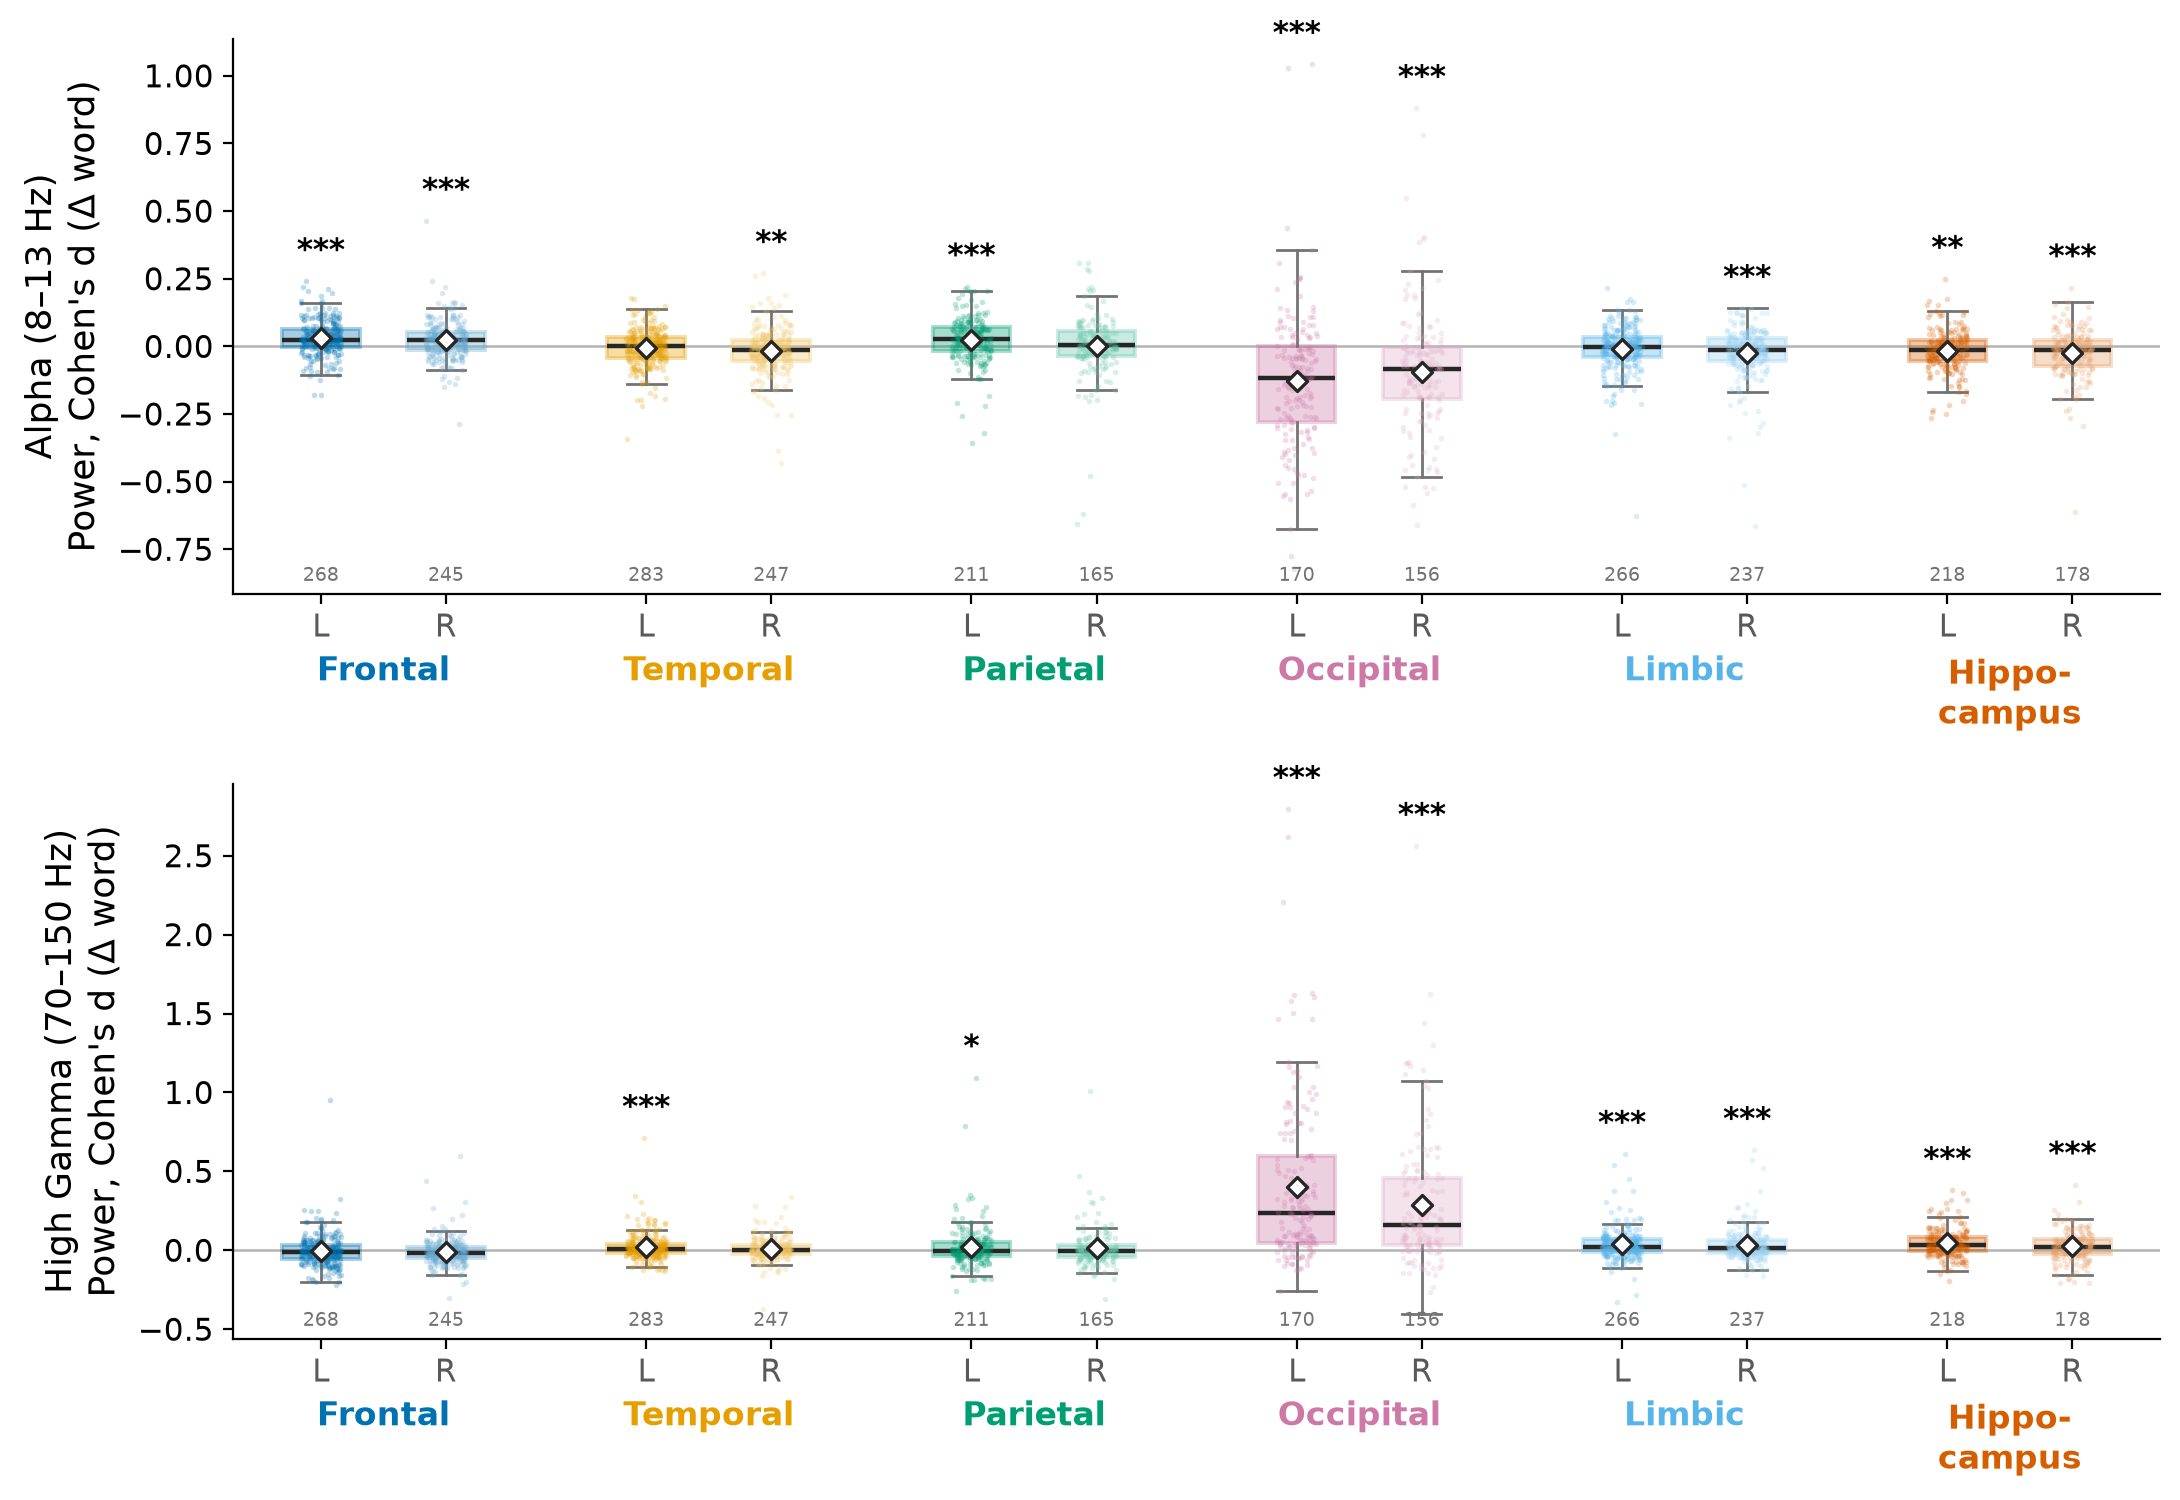
\includegraphics[width=0.75\linewidth]{img/figS1_power_subjects.png}\par\medskip
\textbf{B}\par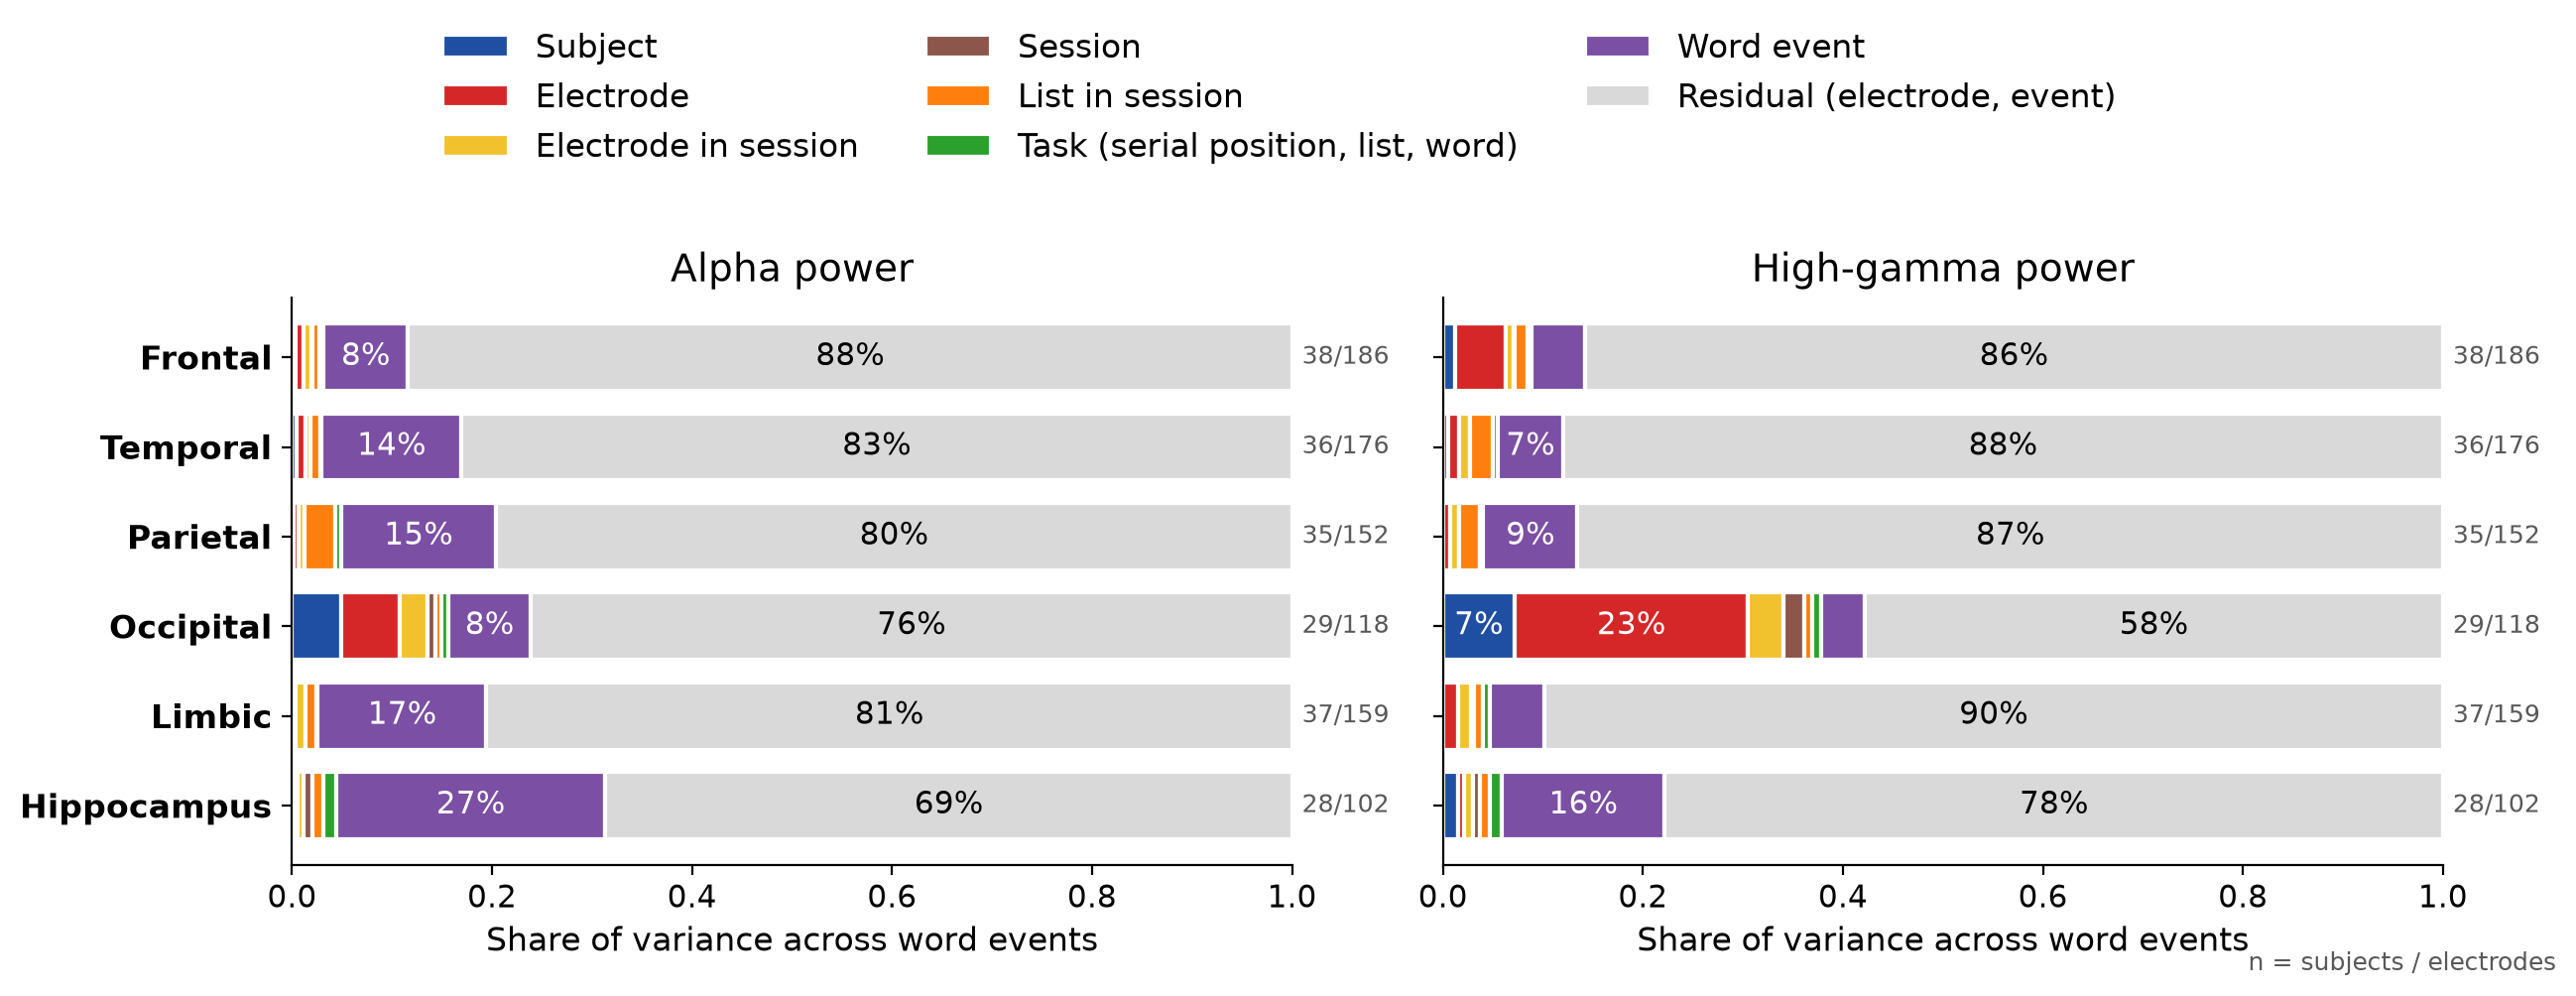
\includegraphics[width=0.9\linewidth]{img/variance_components_power.png}
\caption{(A) Power change at word onset (Cohen's $d$, word on vs.\ off; dots: subjects). (B) Variance components of the response to each word event, one mixed model per lobe (Aim 1; 40-subject pilot). Word event: variance shared by all of a lobe's electrodes on the same word event.}
\label{fig:power}
\end{figure}

\begin{figure}[!h]\centering
\textbf{A}\par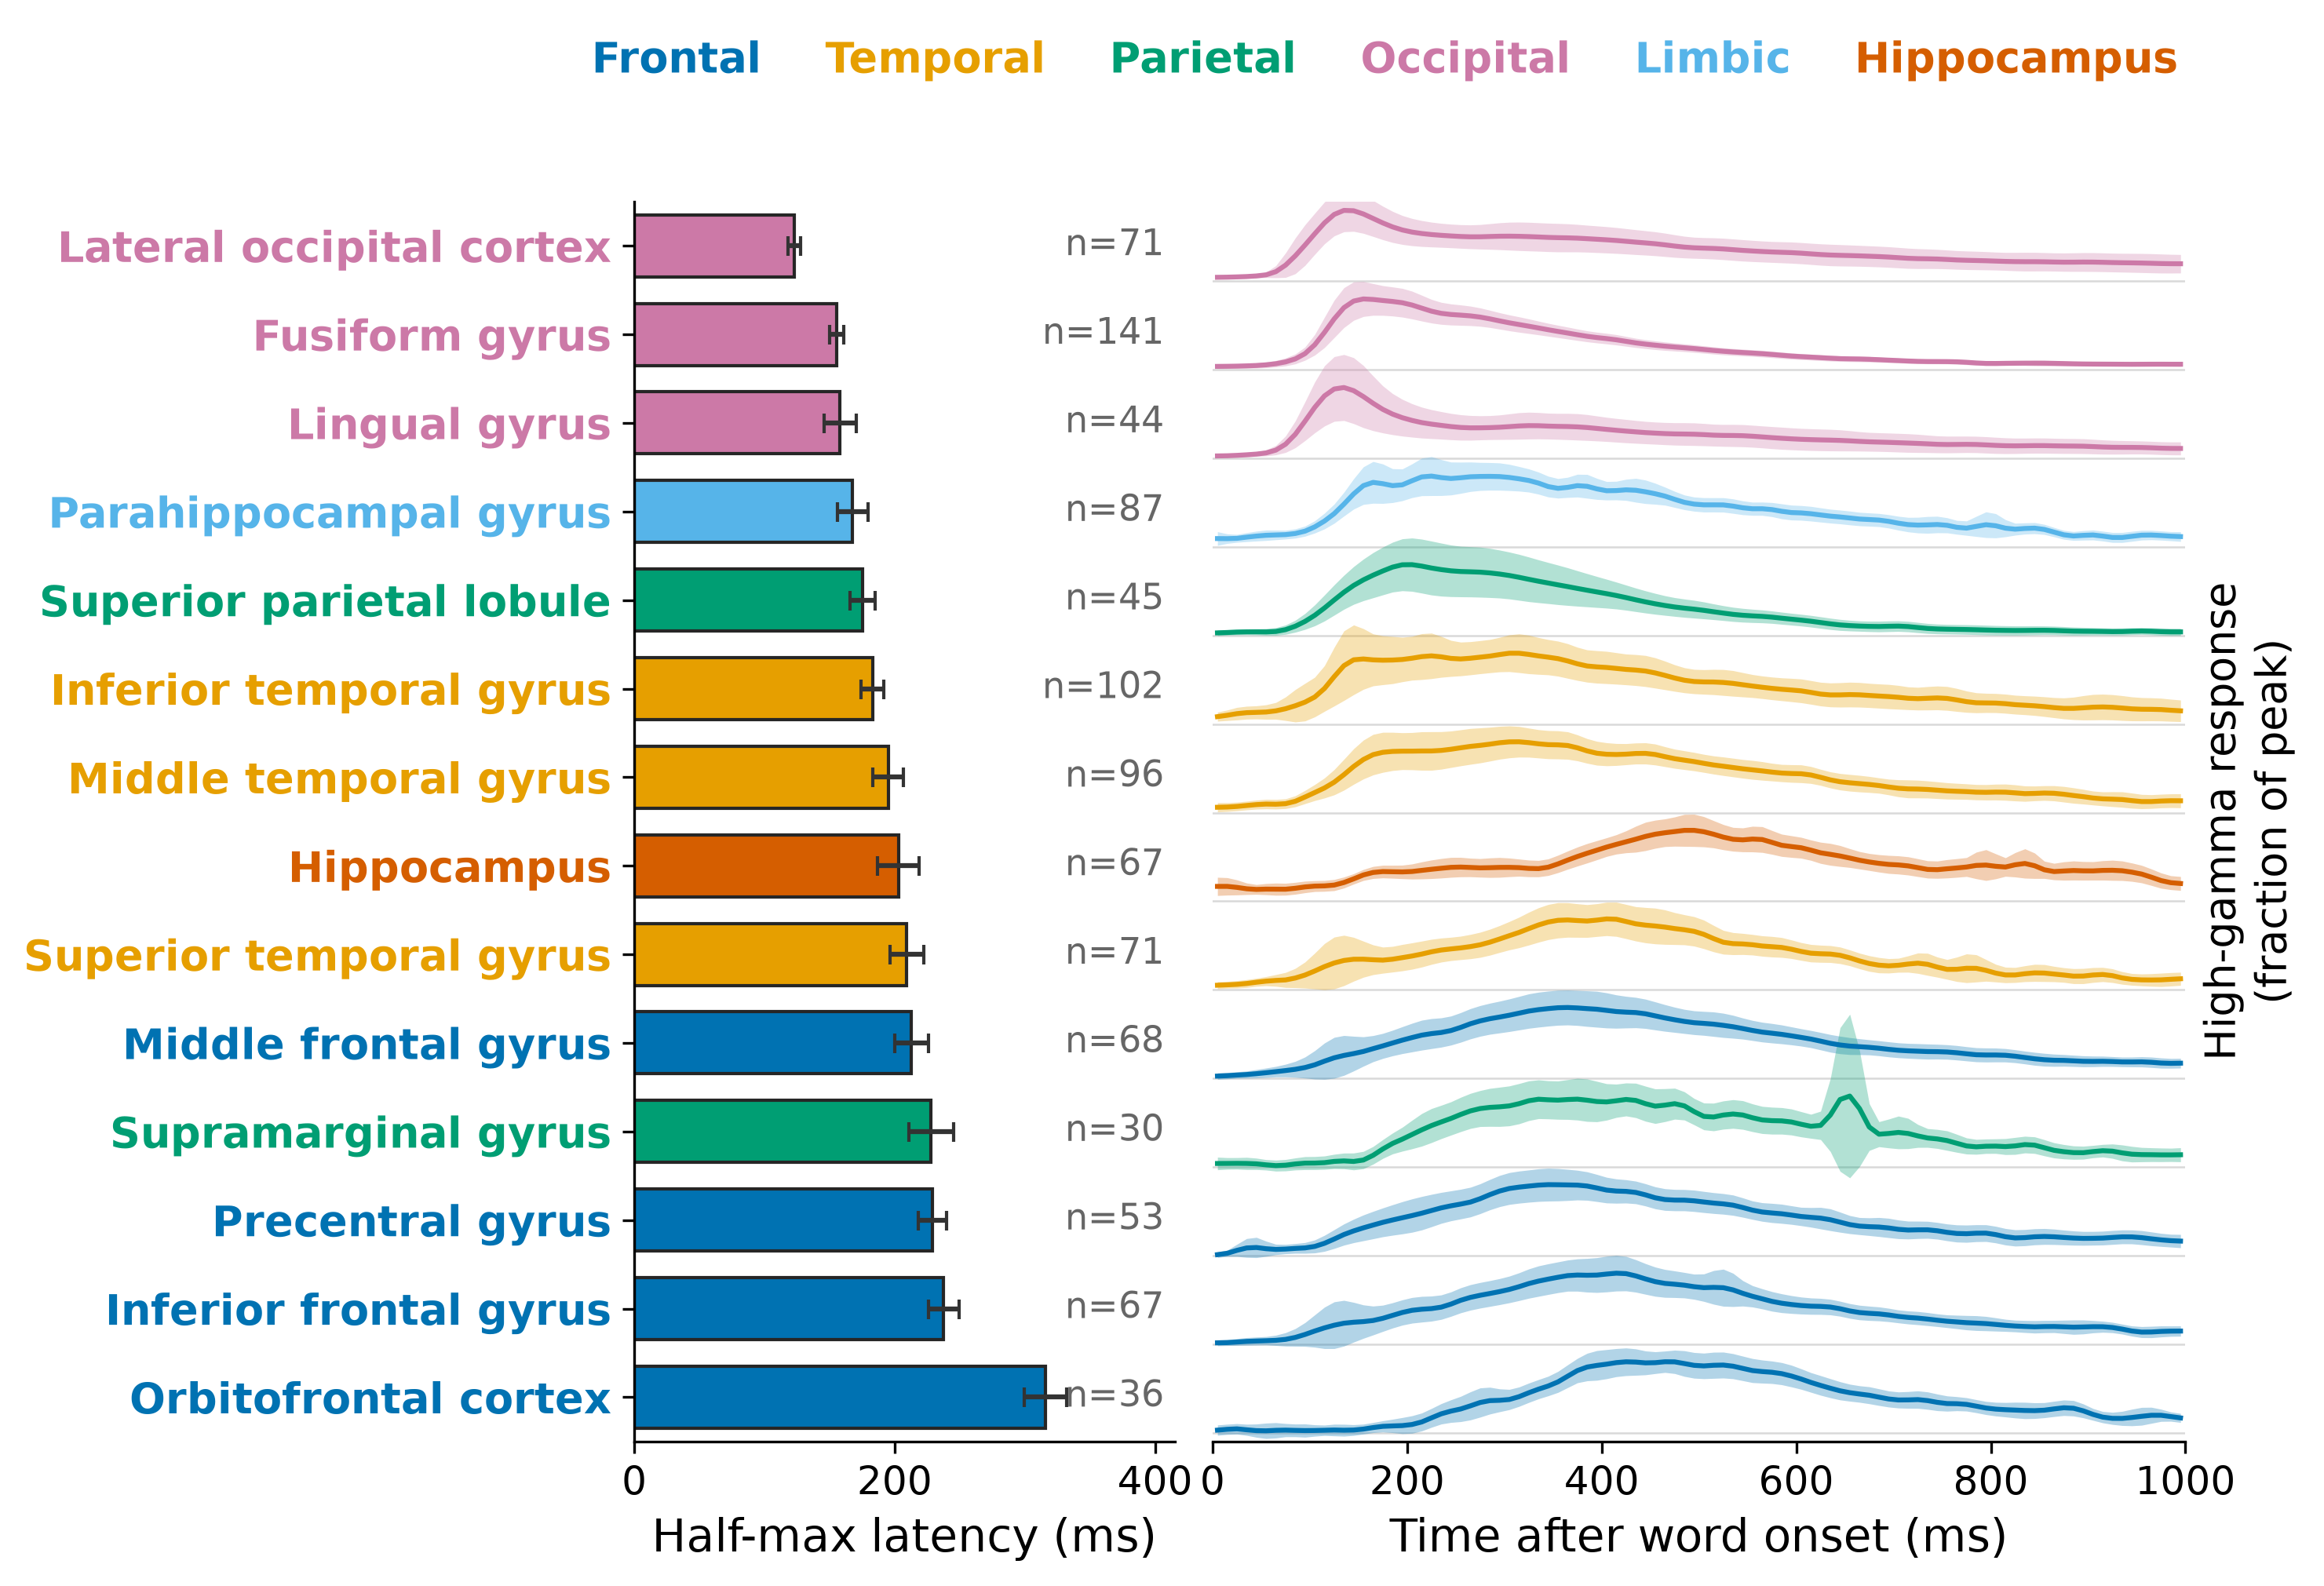
\includegraphics[width=0.75\linewidth]{img/fig4b_latency_fine.png}\par\medskip
\textbf{B}\par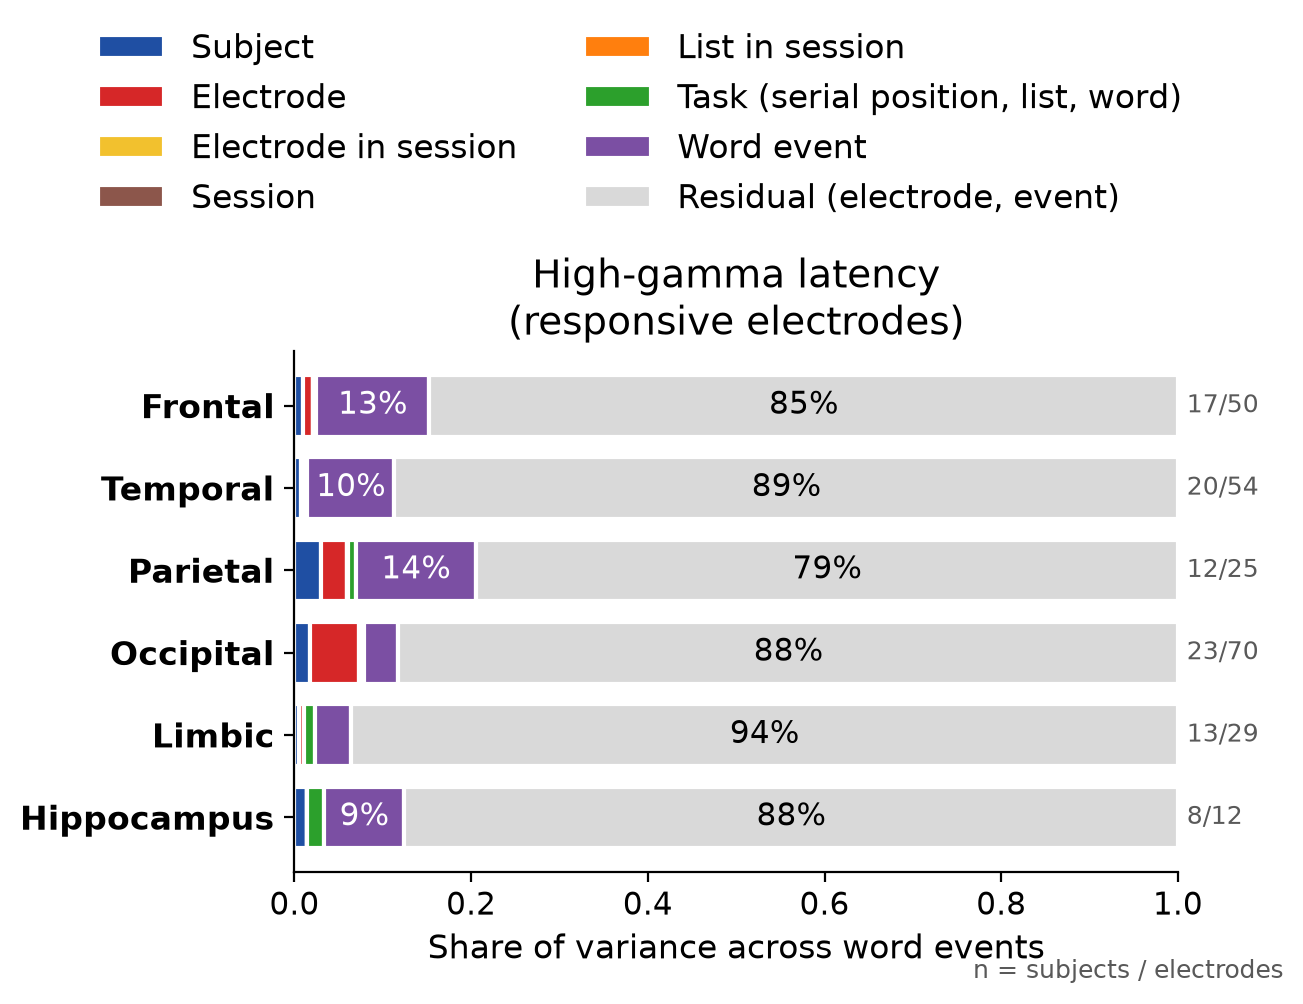
\includegraphics[width=0.5\linewidth]{img/variance_components_latency.png}
\caption{(A) High-gamma half-max latency per region (the supramarginal spike at 650 ms is one artifact word event). (B) Variance components of latency per word event (responsive electrodes; 40-subject pilot).}
\label{fig:latency}
\end{figure}

\begin{figure}[!h]\centering
\textbf{A}\par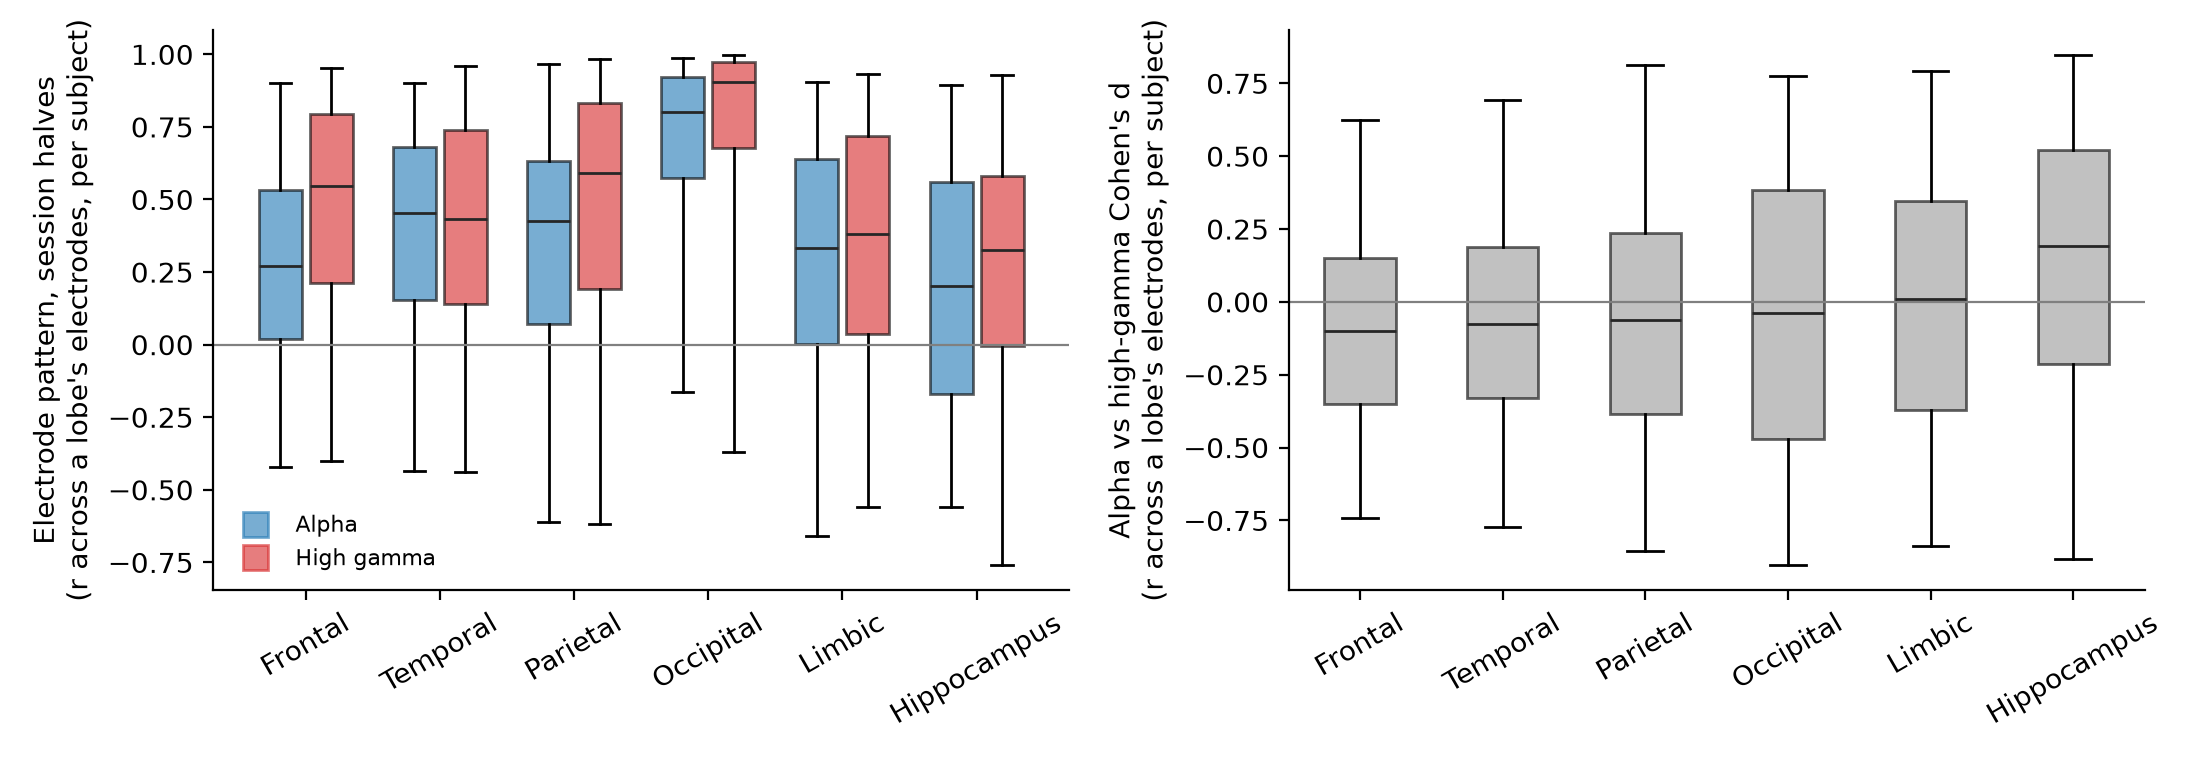
\includegraphics[width=0.6\linewidth]{img/electrode_reliability.png}\par\medskip
\textbf{B}\par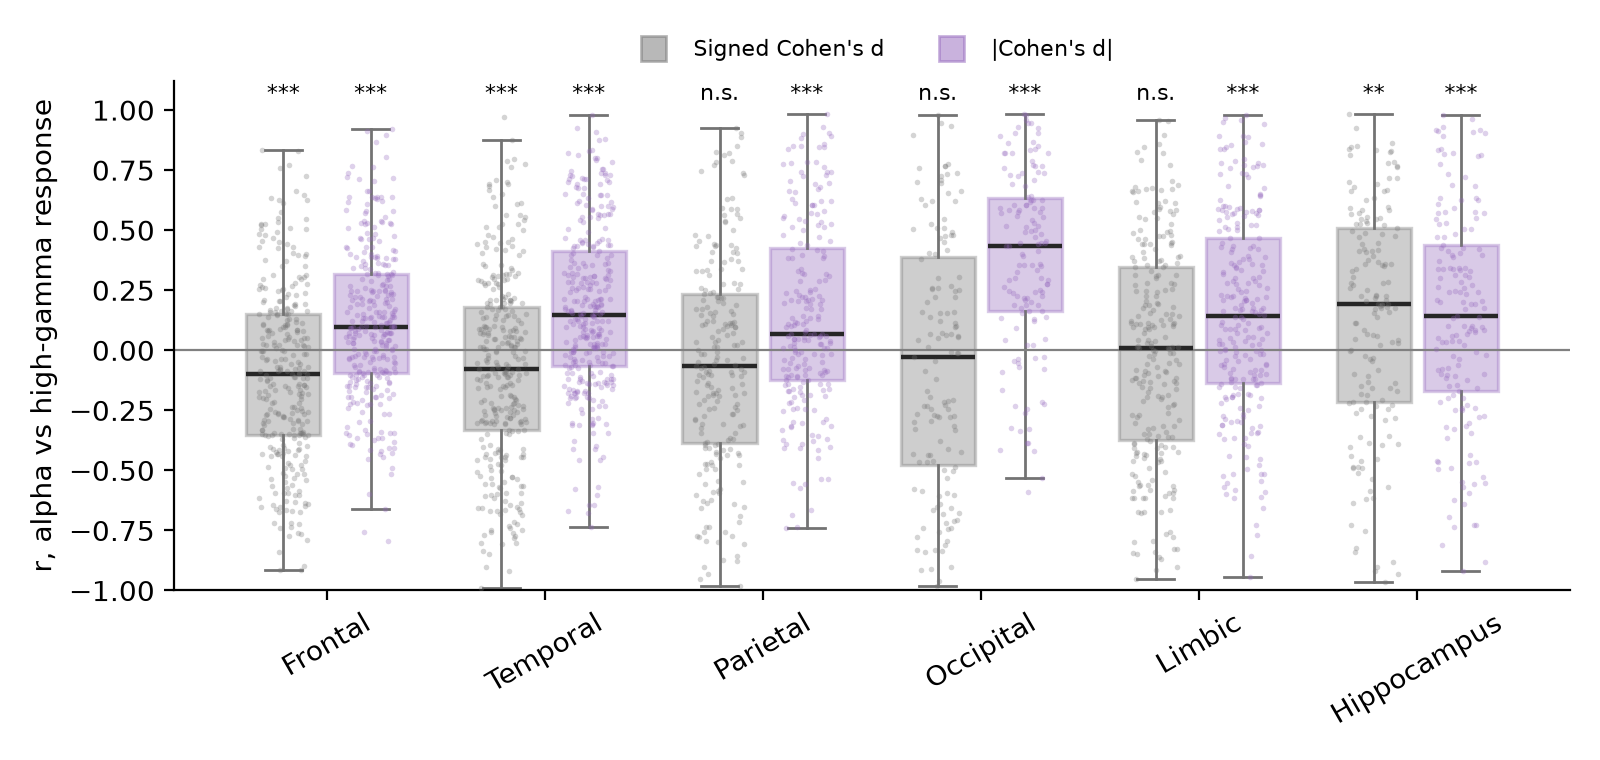
\includegraphics[width=0.75\linewidth]{img/alpha_hg_across_electrodes.png}
\caption{(A) Electrode test-retest: $r$ of electrodes' Cohen's $d$ between session halves (dots: subjects). (B) Alpha vs.\ high gamma across a lobe's electrodes: $r$ of Cohen's $d$ and of $|d|$ per subject (dots); stars: subjects' mean $r$ vs.\ 0, FDR.}
\label{fig:stable}
\end{figure}

\begin{figure}[!h]\centering
\textbf{A}\par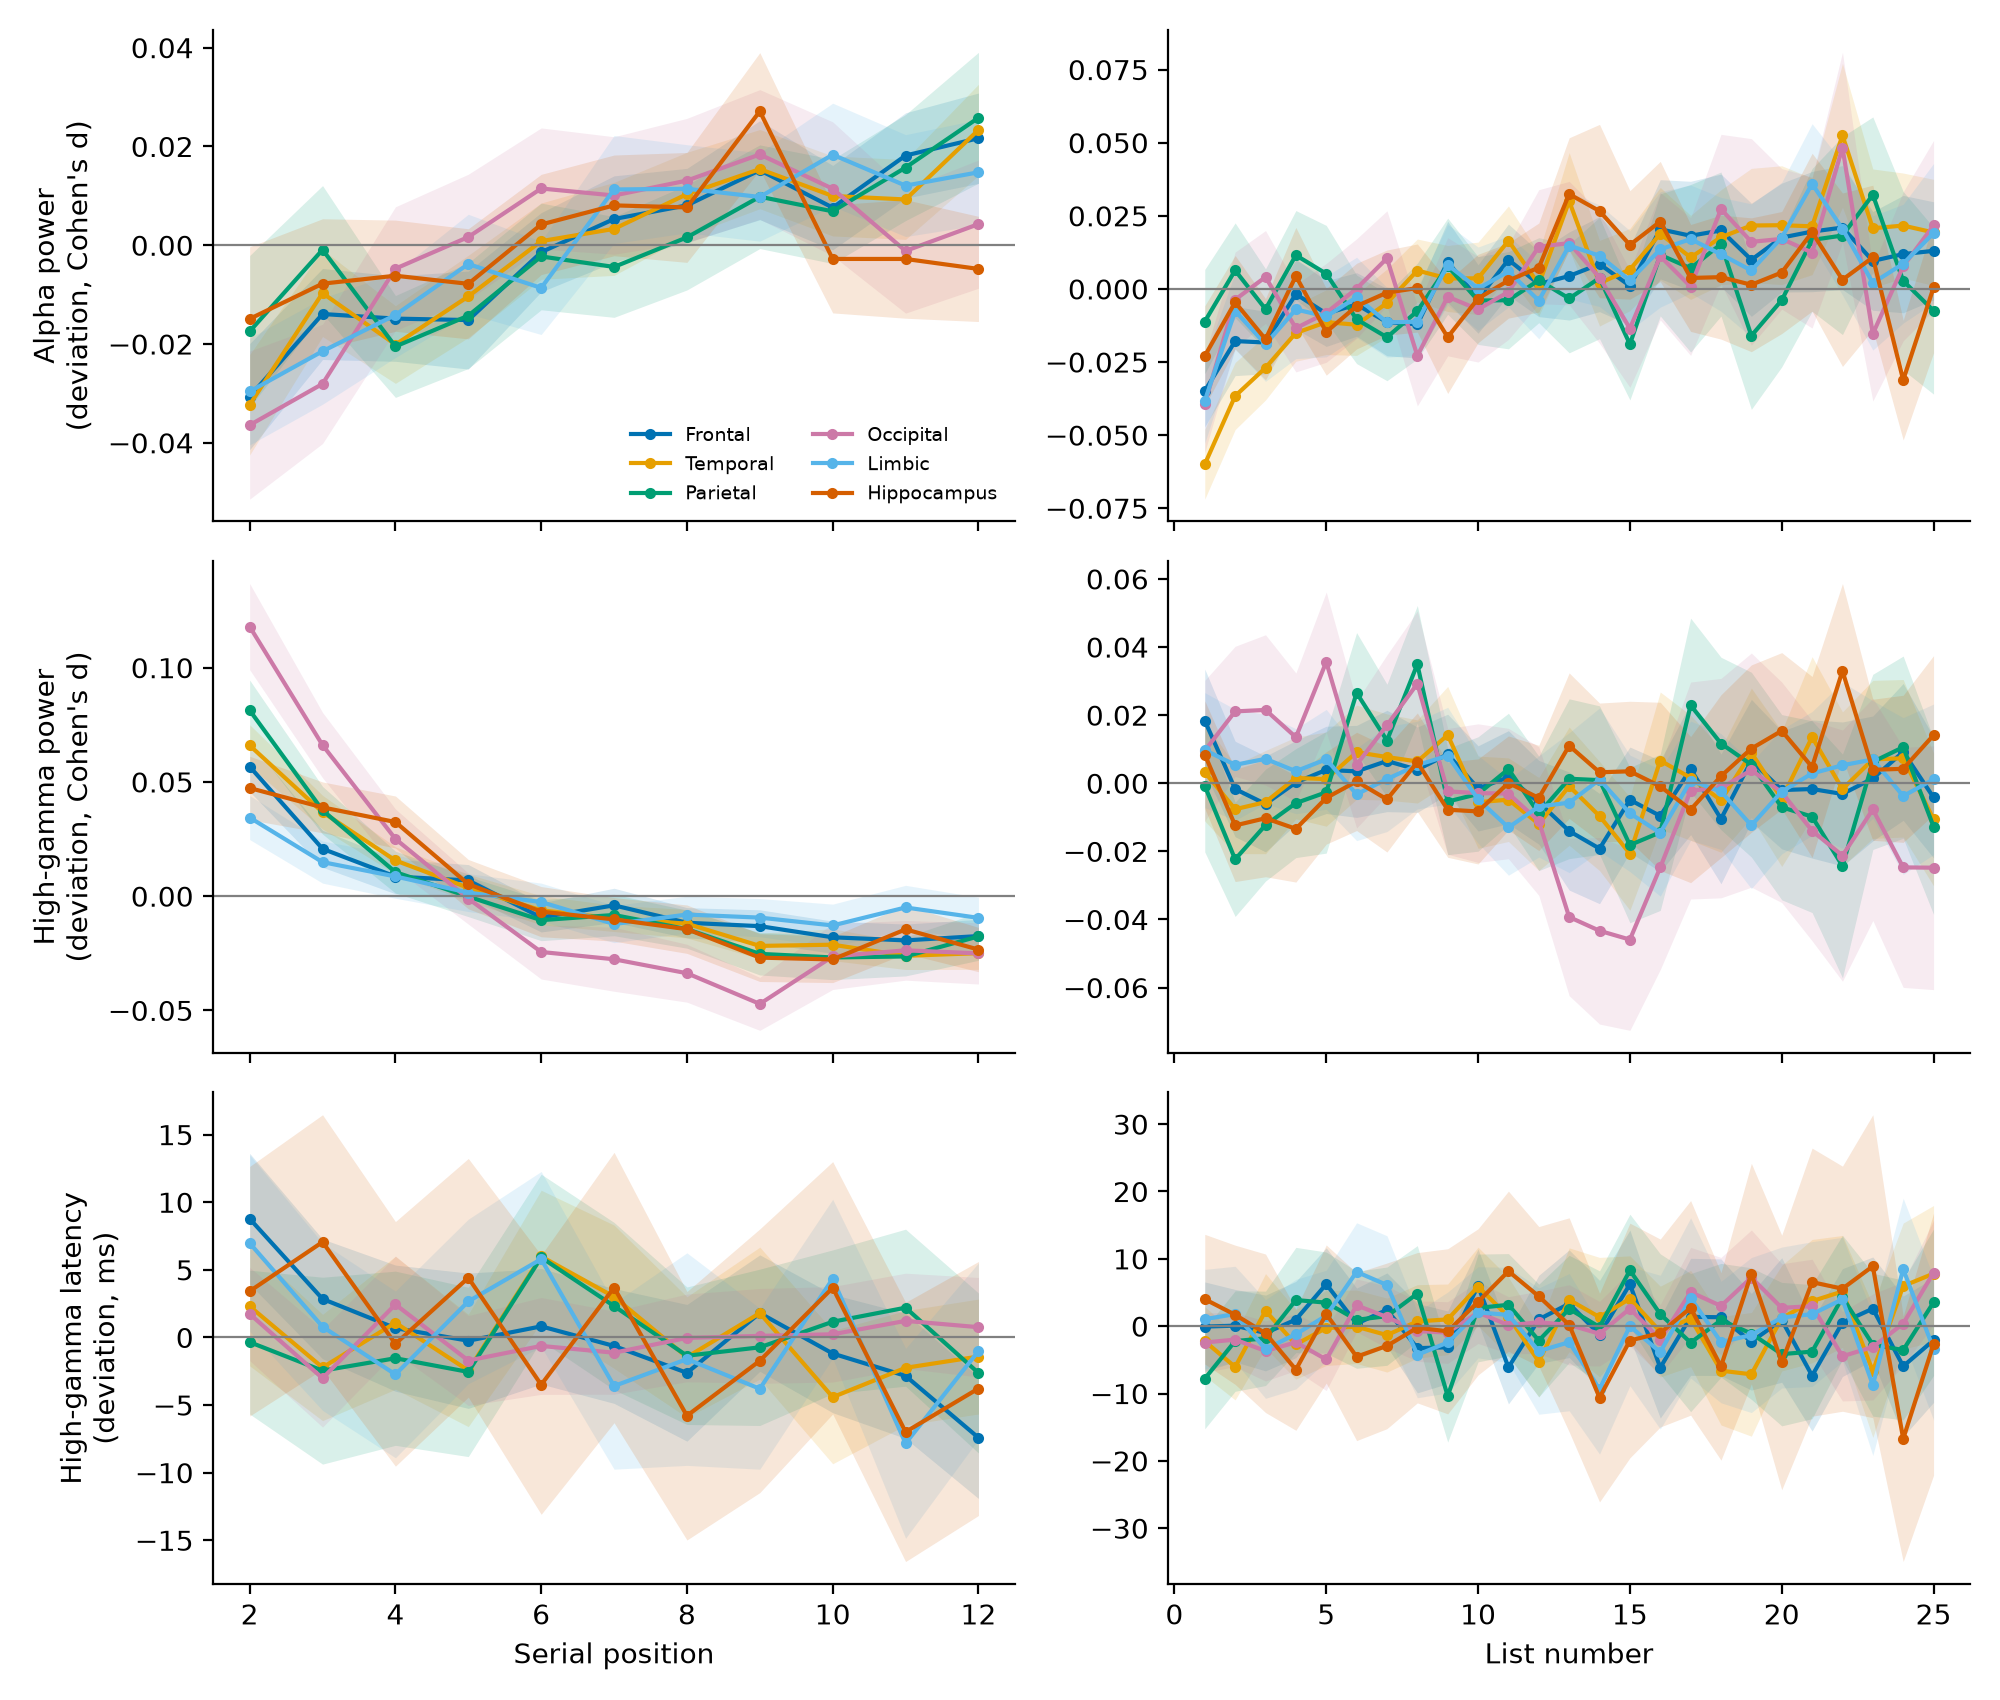
\includegraphics[width=0.8\linewidth]{img/task_effects.png}\par\medskip
\textbf{B}\par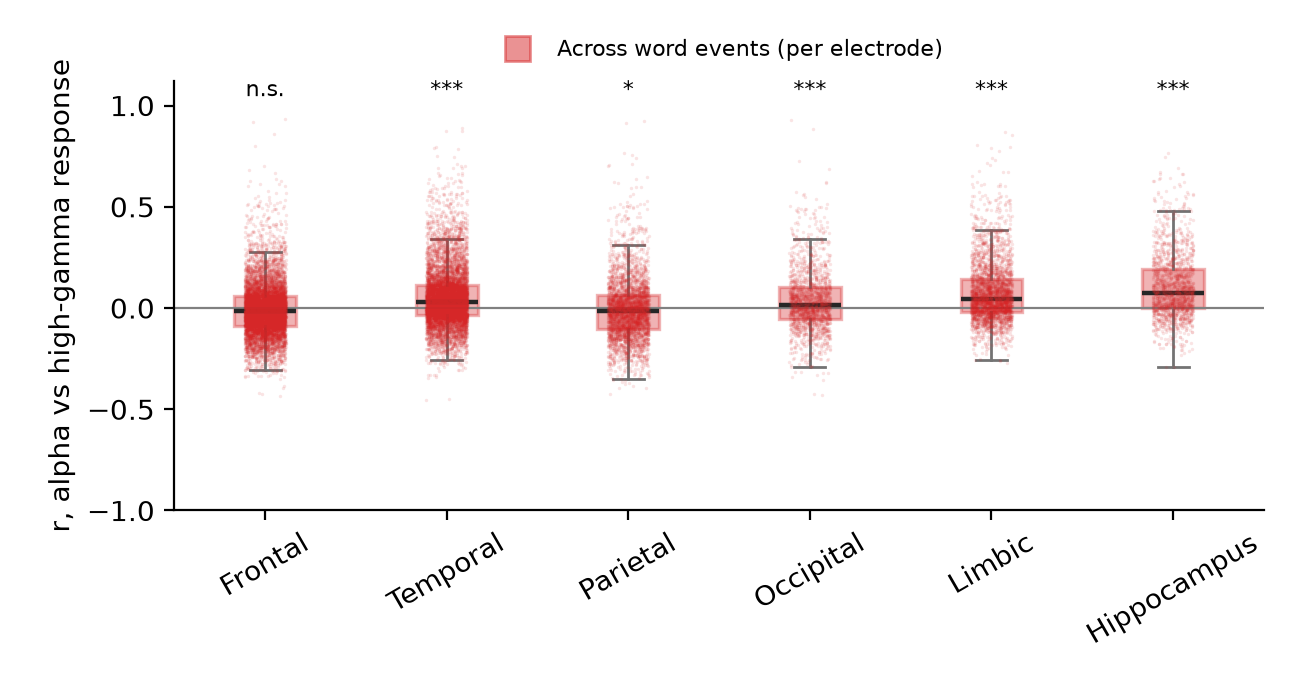
\includegraphics[width=0.65\linewidth]{img/alpha_hg_across_events.png}
\caption{(A) Serial-position and list effects: deviation from each subject's own mean (all electrodes; latency: responsive electrodes); mean and 95\% CI across subjects. (B) Alpha vs.\ high gamma across word events: $r$ per electrode (dots); stars: subjects' mean $r$ vs.\ 0, FDR.}
\label{fig:word}
\end{figure}

\begin{figure}[!h]\centering
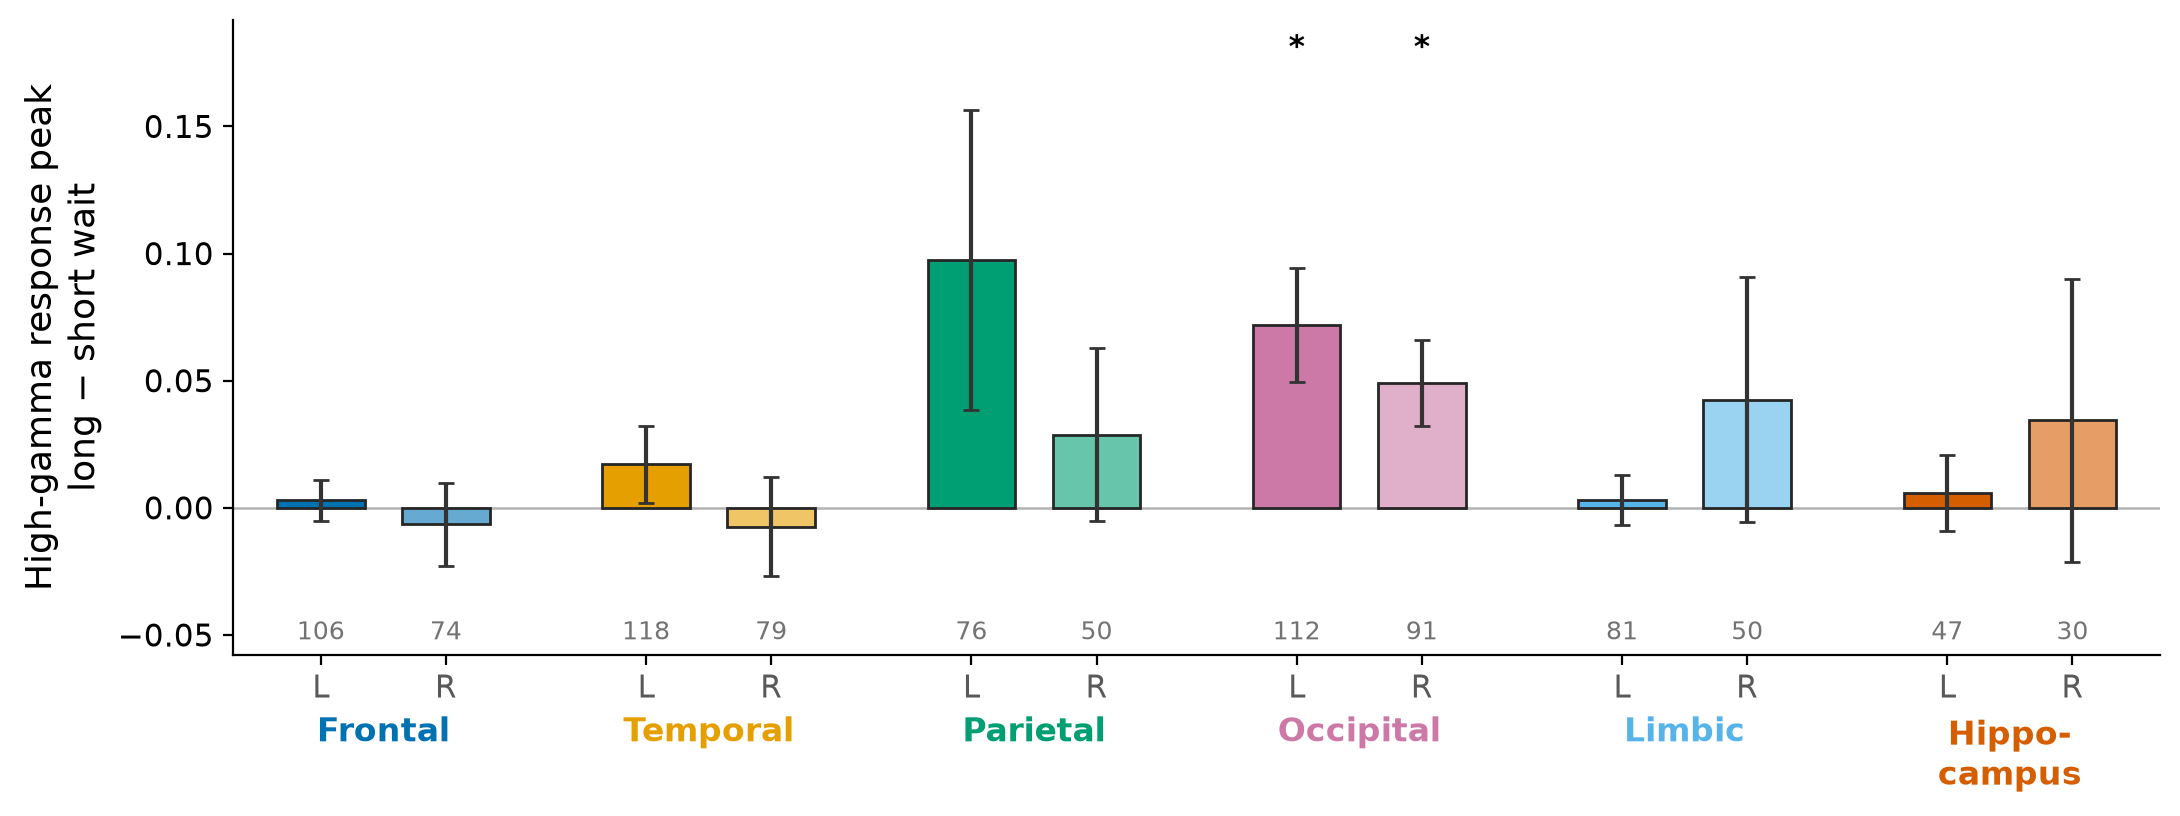
\includegraphics[width=0.7\linewidth]{img/fig9_anticipation.png}
\caption{High-gamma response peak after long vs.\ short blanks, per region (stars: FDR; n: subjects).}
\label{fig:wait}
\end{figure}

\clearpage
\bibliographystyle{apalike}
\bibliography{../paper/refs,extra}
\end{document}
